\documentclass[12pt]{article}

% ---------------- Packages ----------------
\usepackage[a4paper, margin=1in]{geometry}
\usepackage{setspace}
\usepackage{amsmath, amsfonts, amssymb}
\usepackage{graphicx}
\usepackage{fancyhdr}
\usepackage{xcolor}
\usepackage{listings}
\usepackage{titling} % cleaner title formatting
\usepackage{tabularx}
\usepackage{microtype}
\usepackage{enumitem}
\usepackage{subcaption}
\usepackage{float}

% ---------------- Page Setup ----------------
\setstretch{1.2}
\setlist[itemize]{leftmargin=*, itemsep=0.25em, topsep=0.4em}
\setlist[enumerate]{leftmargin=*, itemsep=0.35em, topsep=0.4em}
\captionsetup{font=small, labelfont=bf}

% ---------------- Fancy Header & Footer ----------------

\pagestyle{fancy}
\fancyhf{}

% Header
\fancyhead[L]{\small CSE 4616 -- Wireless Networks}
\fancyhead[R]{\small Islamic University of Technology}

% Footer (Dotted leader line + page number)
\renewcommand{\footrulewidth}{0pt} % remove default line

\newcommand{\dottedfooter}{
    \par\vspace*{4pt}
    \noindent\makebox[\linewidth]{\dotfill}%
}

\fancyfoot[C]{\dottedfooter\\[0pt] \thepage}

% ---------------- Custom Title Page ----------------
\newcommand{\maketitlepage}{
    \begin{titlepage}
        \centering
        \vspace*{1.5cm}

        % University Name
        {\Huge \textbf{Islamic University of Technology}}\\[12pt]
        {\Large Department of Computer Science and Engineering}\\[25pt]

        % Divider
        \rule{0.85\textwidth}{0.6pt} \\[14pt]

        % Main Title Block
        {\LARGE \textbf{CSE 4616 -- Wireless Networks}}\\[8pt]
        {\Large \textbf{Lab 01: Introduction to OMNeT++ and INET}}\\[6pt]

        \rule{0.85\textwidth}{0.6pt} \\[40pt]

        % Date Box
        \begin{tabular}{rl}
            \textbf{Date:} & \today
        \end{tabular}

        \vspace{4cm}

        % Right-Aligned Submission Block
        \hfill
        \begin{minipage}{0.50\textwidth}
            \raggedleft
            \textbf{Submitted by:} \\
            Obidit Islam \\
            \textbf{Student ID:} 220041154
        \end{minipage}

        \vfill
    \end{titlepage}
}

% ---------------- Document Starts ----------------
\begin{document}

\maketitlepage

\section{Introduction}
The objective of this lab report is to apply and document modifications to the INET example network in OMNeT++ and analyze the resulting simulation behavior for each task.

\section{In-Lab Assessment Tasks}
\subsection{General Instructions}
\begin{itemize}
    \item All tasks are based on the prebuilt sample network WiredAndWirelessHostsWithAP.
    \item Each task builds on the original NED and INI files unless stated otherwise.
    \item Name your files clearly: TaskX YourStudentID.ned and TaskX YourStudentID.ini.
    \item Take Qtenv screenshots while the simulation is running (packets visible) unless the task states otherwise.
    \item Write explanations in the report or as comments inside the submitted files.
\end{itemize}

\subsection{Task 01: Modify Traffic Parameters}
\textbf{Background:} Modify the traffic parameters in the INI file to simulate a higher-load scenario and observe the difference in Qtenv.

\textbf{Required Modifications (INI file only):}
\begin{enumerate}
    \item Change the packet size from 100B to 500B for all sending apps.
    \item Change the send interval from 1s to 0.5s for all sending apps.
    \item Change the stop time of all sending apps from 300s to 350s.
    \item Change the overall simulation time limit from 400s to 500s.
\end{enumerate}

\textbf{Analysis Questions:}
\begin{enumerate}
    \item How many packets per second does each host generate in total after your modification? Show your calculation.\\
    \textbf{Answer:}\\
    Each host has 2 senders (app[1] and app[2]). With sendInterval = 0.5s, each sender sends 2 packets/second.\\
    Total per host = 2 senders $\times$ 2 packets/s = 4 packets/second.
    \item What is the total data rate (bytes per second) generated by wiredHost1 after the modification?\\
    \textbf{Answer:}\\
    wiredHost1 has 2 sending apps, each sending at 2 packets/s $\times$ 500B/packet.\\
    Data rate = 2 $\times$ 2 $\times$ 500 = 2,000 bytes/second = 2 KB/s.
    \item In Qtenv, did you notice any visual difference compared to the original simulation? Describe what you observed.\\
    \textbf{Answer:}\\
    I observed noticeably more packet animations flying between nodes. Packets are larger (500B vs 100B) and sent twice as often (every 0.5s vs 1s), so the links appear busier. The simulation also runs longer (to t = 500 s).
    
    \begin{figure}[H]
        \centering
        \begin{subfigure}{0.9\linewidth}
            \centering
            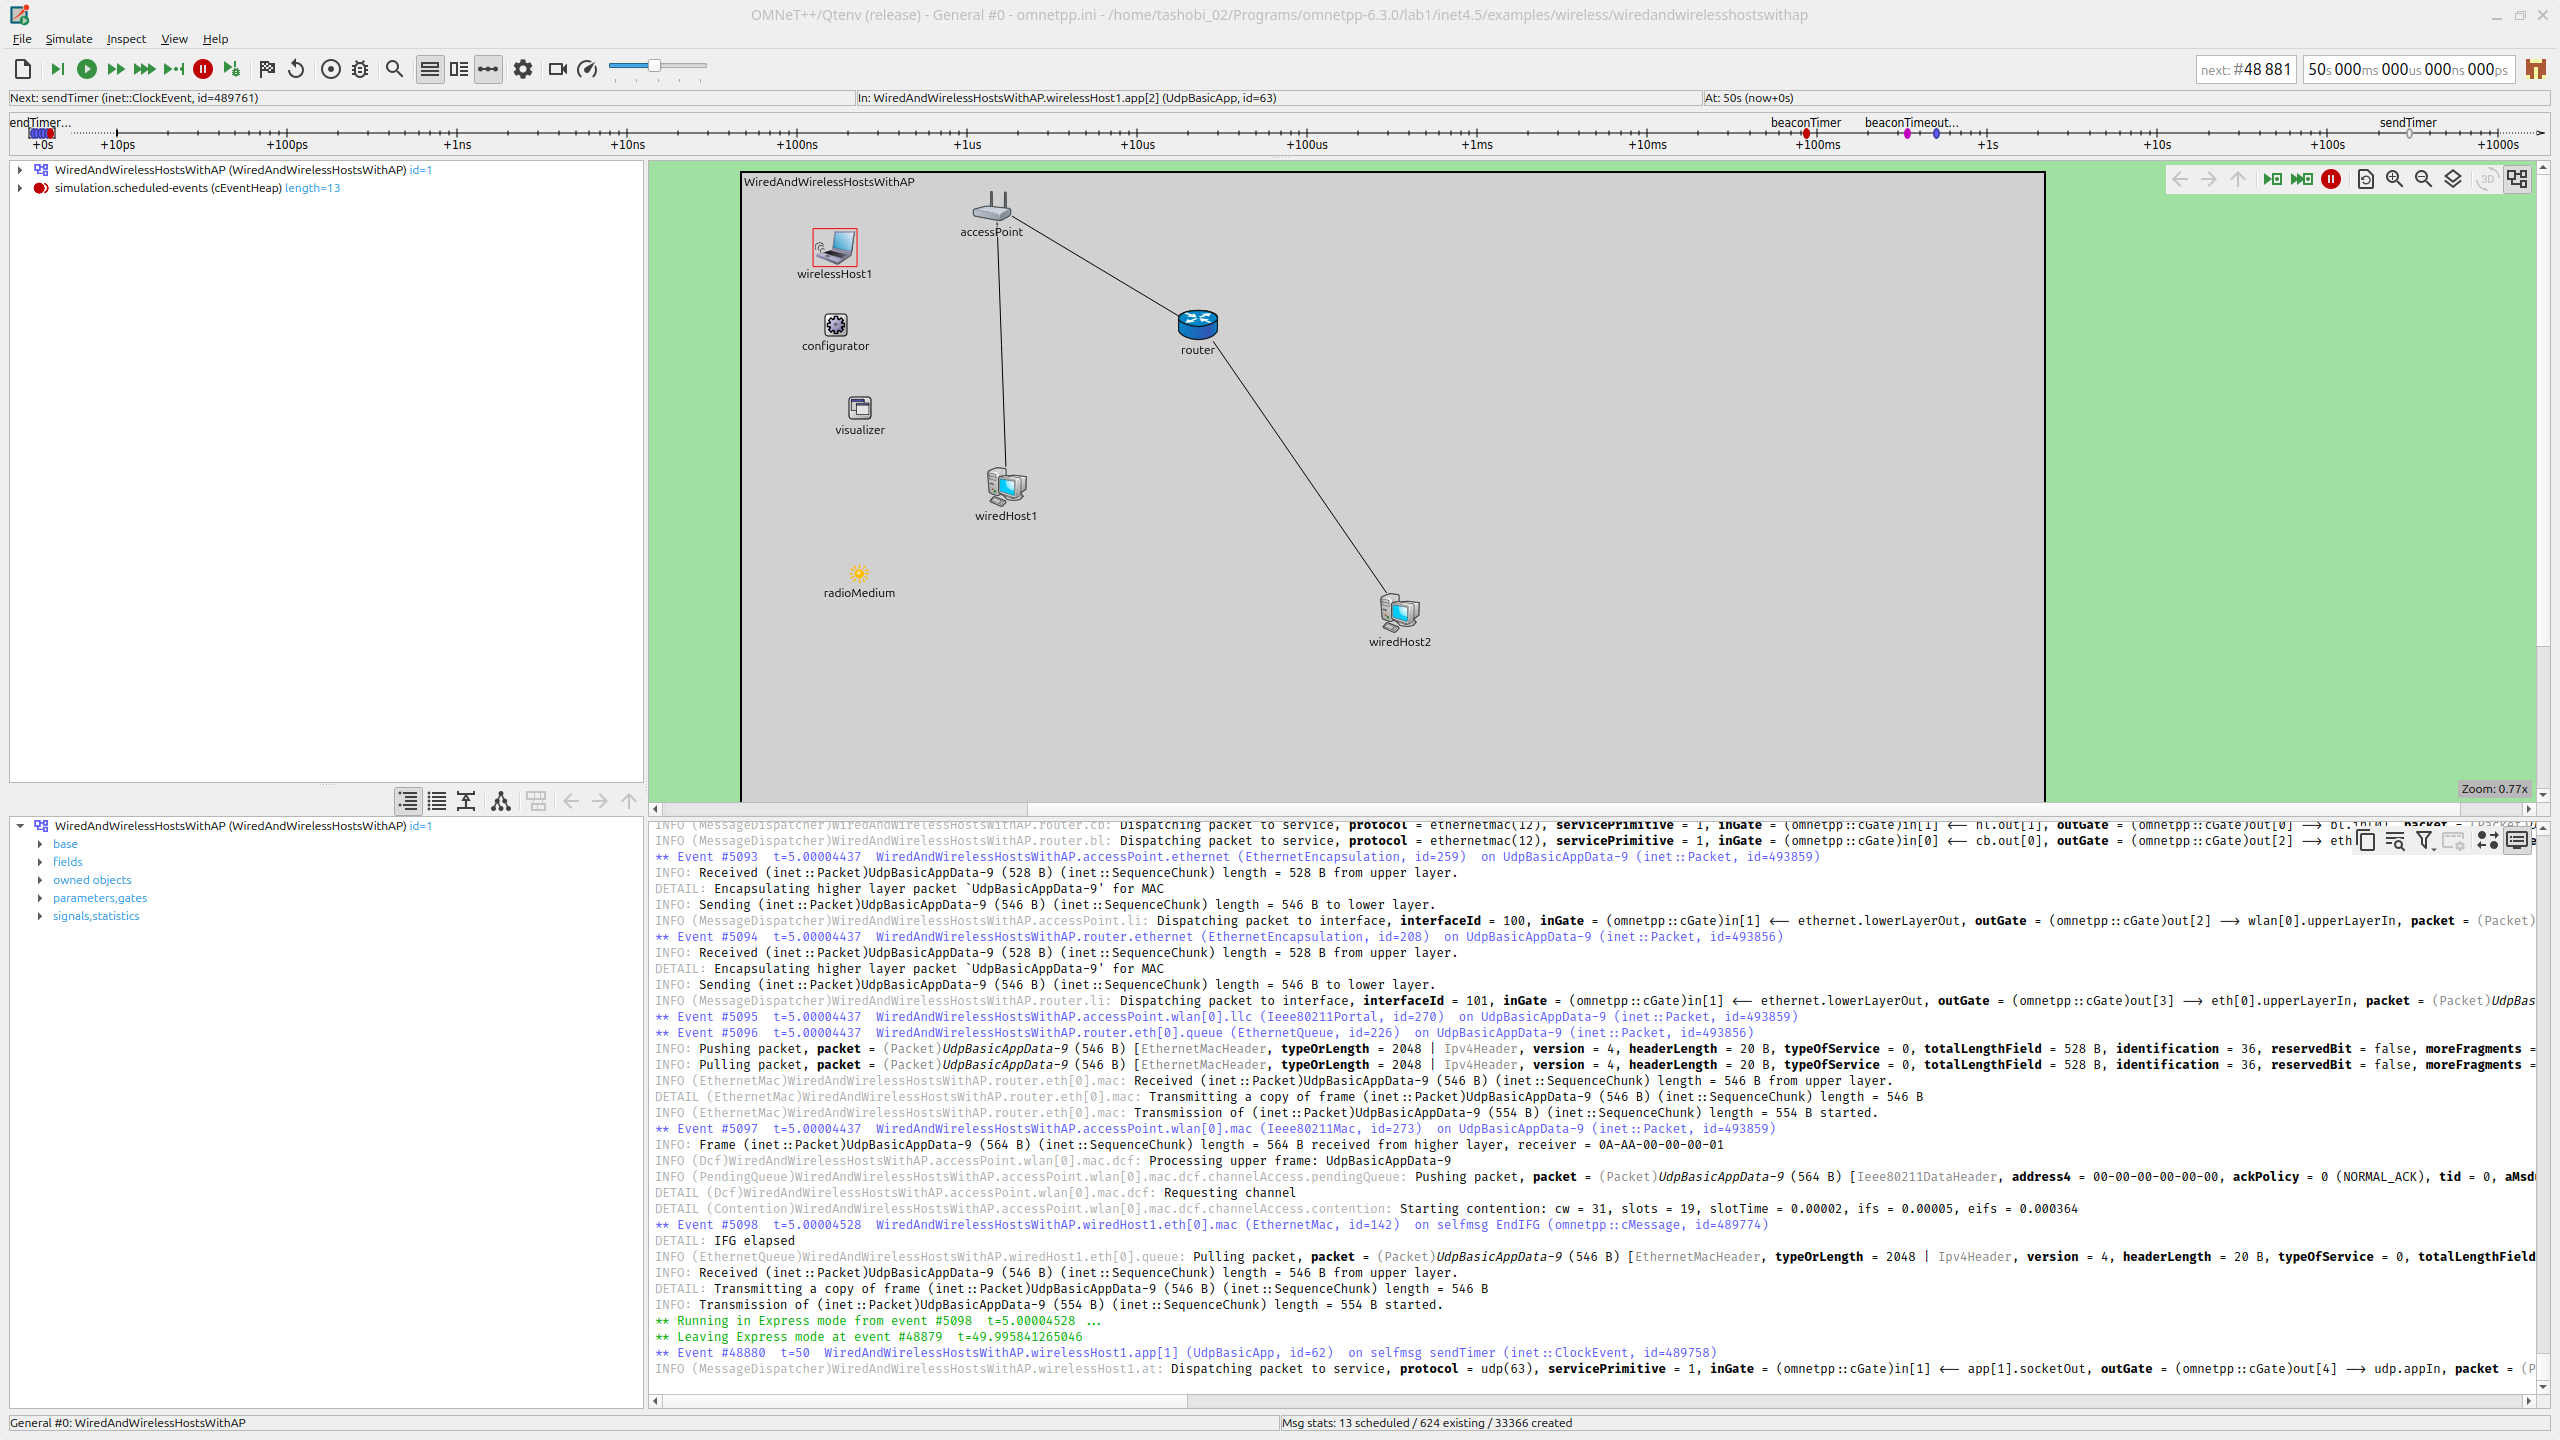
\includegraphics[width=\linewidth]{Figures/fig1.png}
            \caption{t = 50 s}
        \end{subfigure}
        \vspace{6pt}
        \begin{subfigure}{0.9\linewidth}
            \centering
            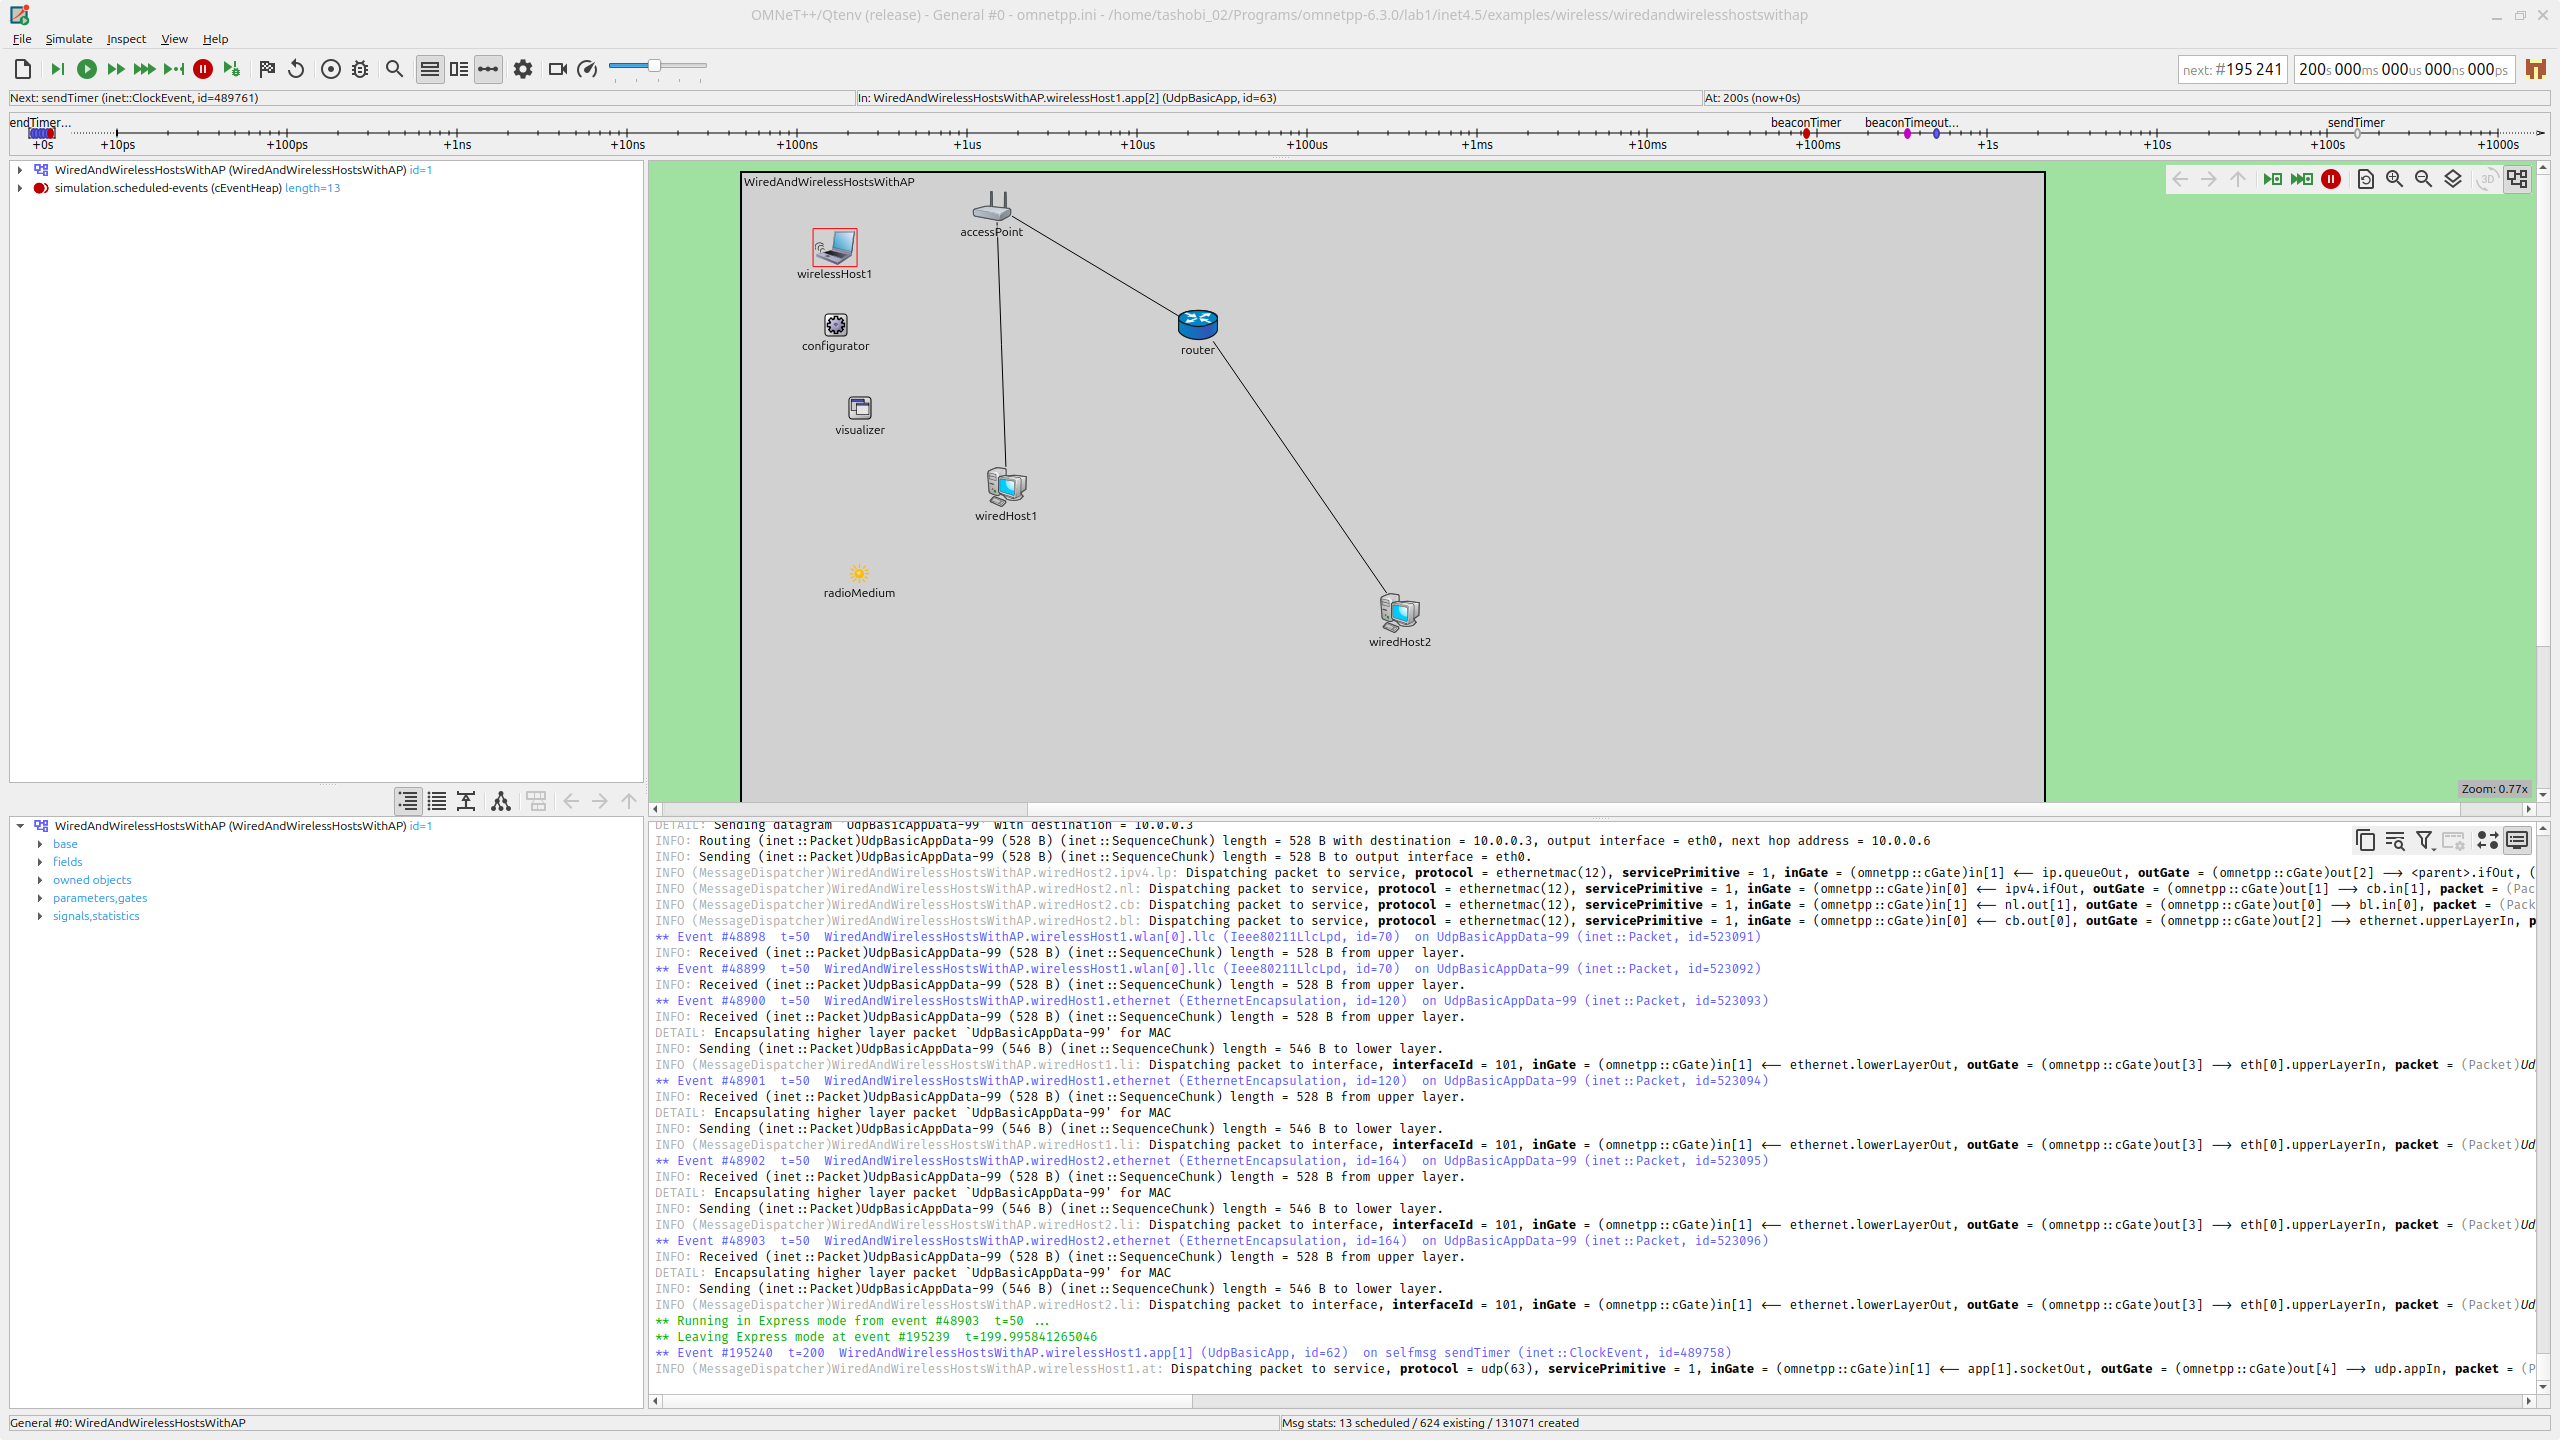
\includegraphics[width=\linewidth]{Figures/fig2.png}
            \caption{t = 200 s}
        \end{subfigure}
        \caption{Qtenv screenshots for Task 01.}
    \end{figure}

\end{enumerate}



\subsection{Task 02: Add a Second Wireless Host}
\textbf{Background:} Add a second wireless host and update traffic so all hosts exchange packets.

\textbf{Required Modifications (NED file):}
\begin{enumerate}
    \item Add a new submodule wirelessHost2 of type WirelessHost at @display("p=62,140").
    \item No new cable connections are needed; wirelessHost2 connects wirelessly via the existing radioMedium.
\end{enumerate}

\textbf{Required Modifications (INI file):}
\begin{enumerate}
    \item Verify that **.*Host*.numApps = 3 applies to wirelessHost2 and explain why in your report.
    \item Add destination address lines so that wirelessHost2 app[1] sends to wiredHost1 and app[2] sends to wirelessHost1.
    \item Update wiredHost1 app[2] destination from "wiredHost2" to "wirelessHost2".
\end{enumerate}

\textbf{Analysis Questions:}
\begin{enumerate}
    \item Draw the updated traffic map (who sends to whom) after your modifications. Use arrows between host names.\\
    \textbf{Answer:}\\
    wiredHost1 $\rightarrow$ (app1) $\rightarrow$ wirelessHost1\\
    wiredHost1 $\rightarrow$ (app2) $\rightarrow$ wirelessHost2\\
    wiredHost2 $\rightarrow$ (app1) $\rightarrow$ wirelessHost1\\
    wiredHost2 $\rightarrow$ (app2) $\rightarrow$ wiredHost1\\
    wirelessHost1 $\rightarrow$ (app1) $\rightarrow$ wiredHost1\\
    wirelessHost1 $\rightarrow$ (app2) $\rightarrow$ wiredHost2\\
    wirelessHost2 $\rightarrow$ (app1) $\rightarrow$ wiredHost1\\
    wirelessHost2 $\rightarrow$ (app2) $\rightarrow$ wirelessHost1
    \item Why does wirelessHost2 not need a new cable connection in the NED file? Explain the role of radioMedium.\\
    \textbf{Answer:}\\
    The radioMedium module acts as the simulated wireless medium. Every module of type WirelessHost or AccessPoint automatically connects to it through its internal wireless radio, not through explicit cable declarations. The radioMedium is like the air itself -- you do not plug into air with a cable. This is the fundamental difference between wired and wireless in OMNeT++/INET.
    \item In Qtenv, can you identify wirelessHost2 on the canvas? Describe its position relative to the access point.\\
    \textbf{Answer:}\\
    Yes, I can identify it. The screenshot is given below.
    \begin{figure}[H]
        \centering
        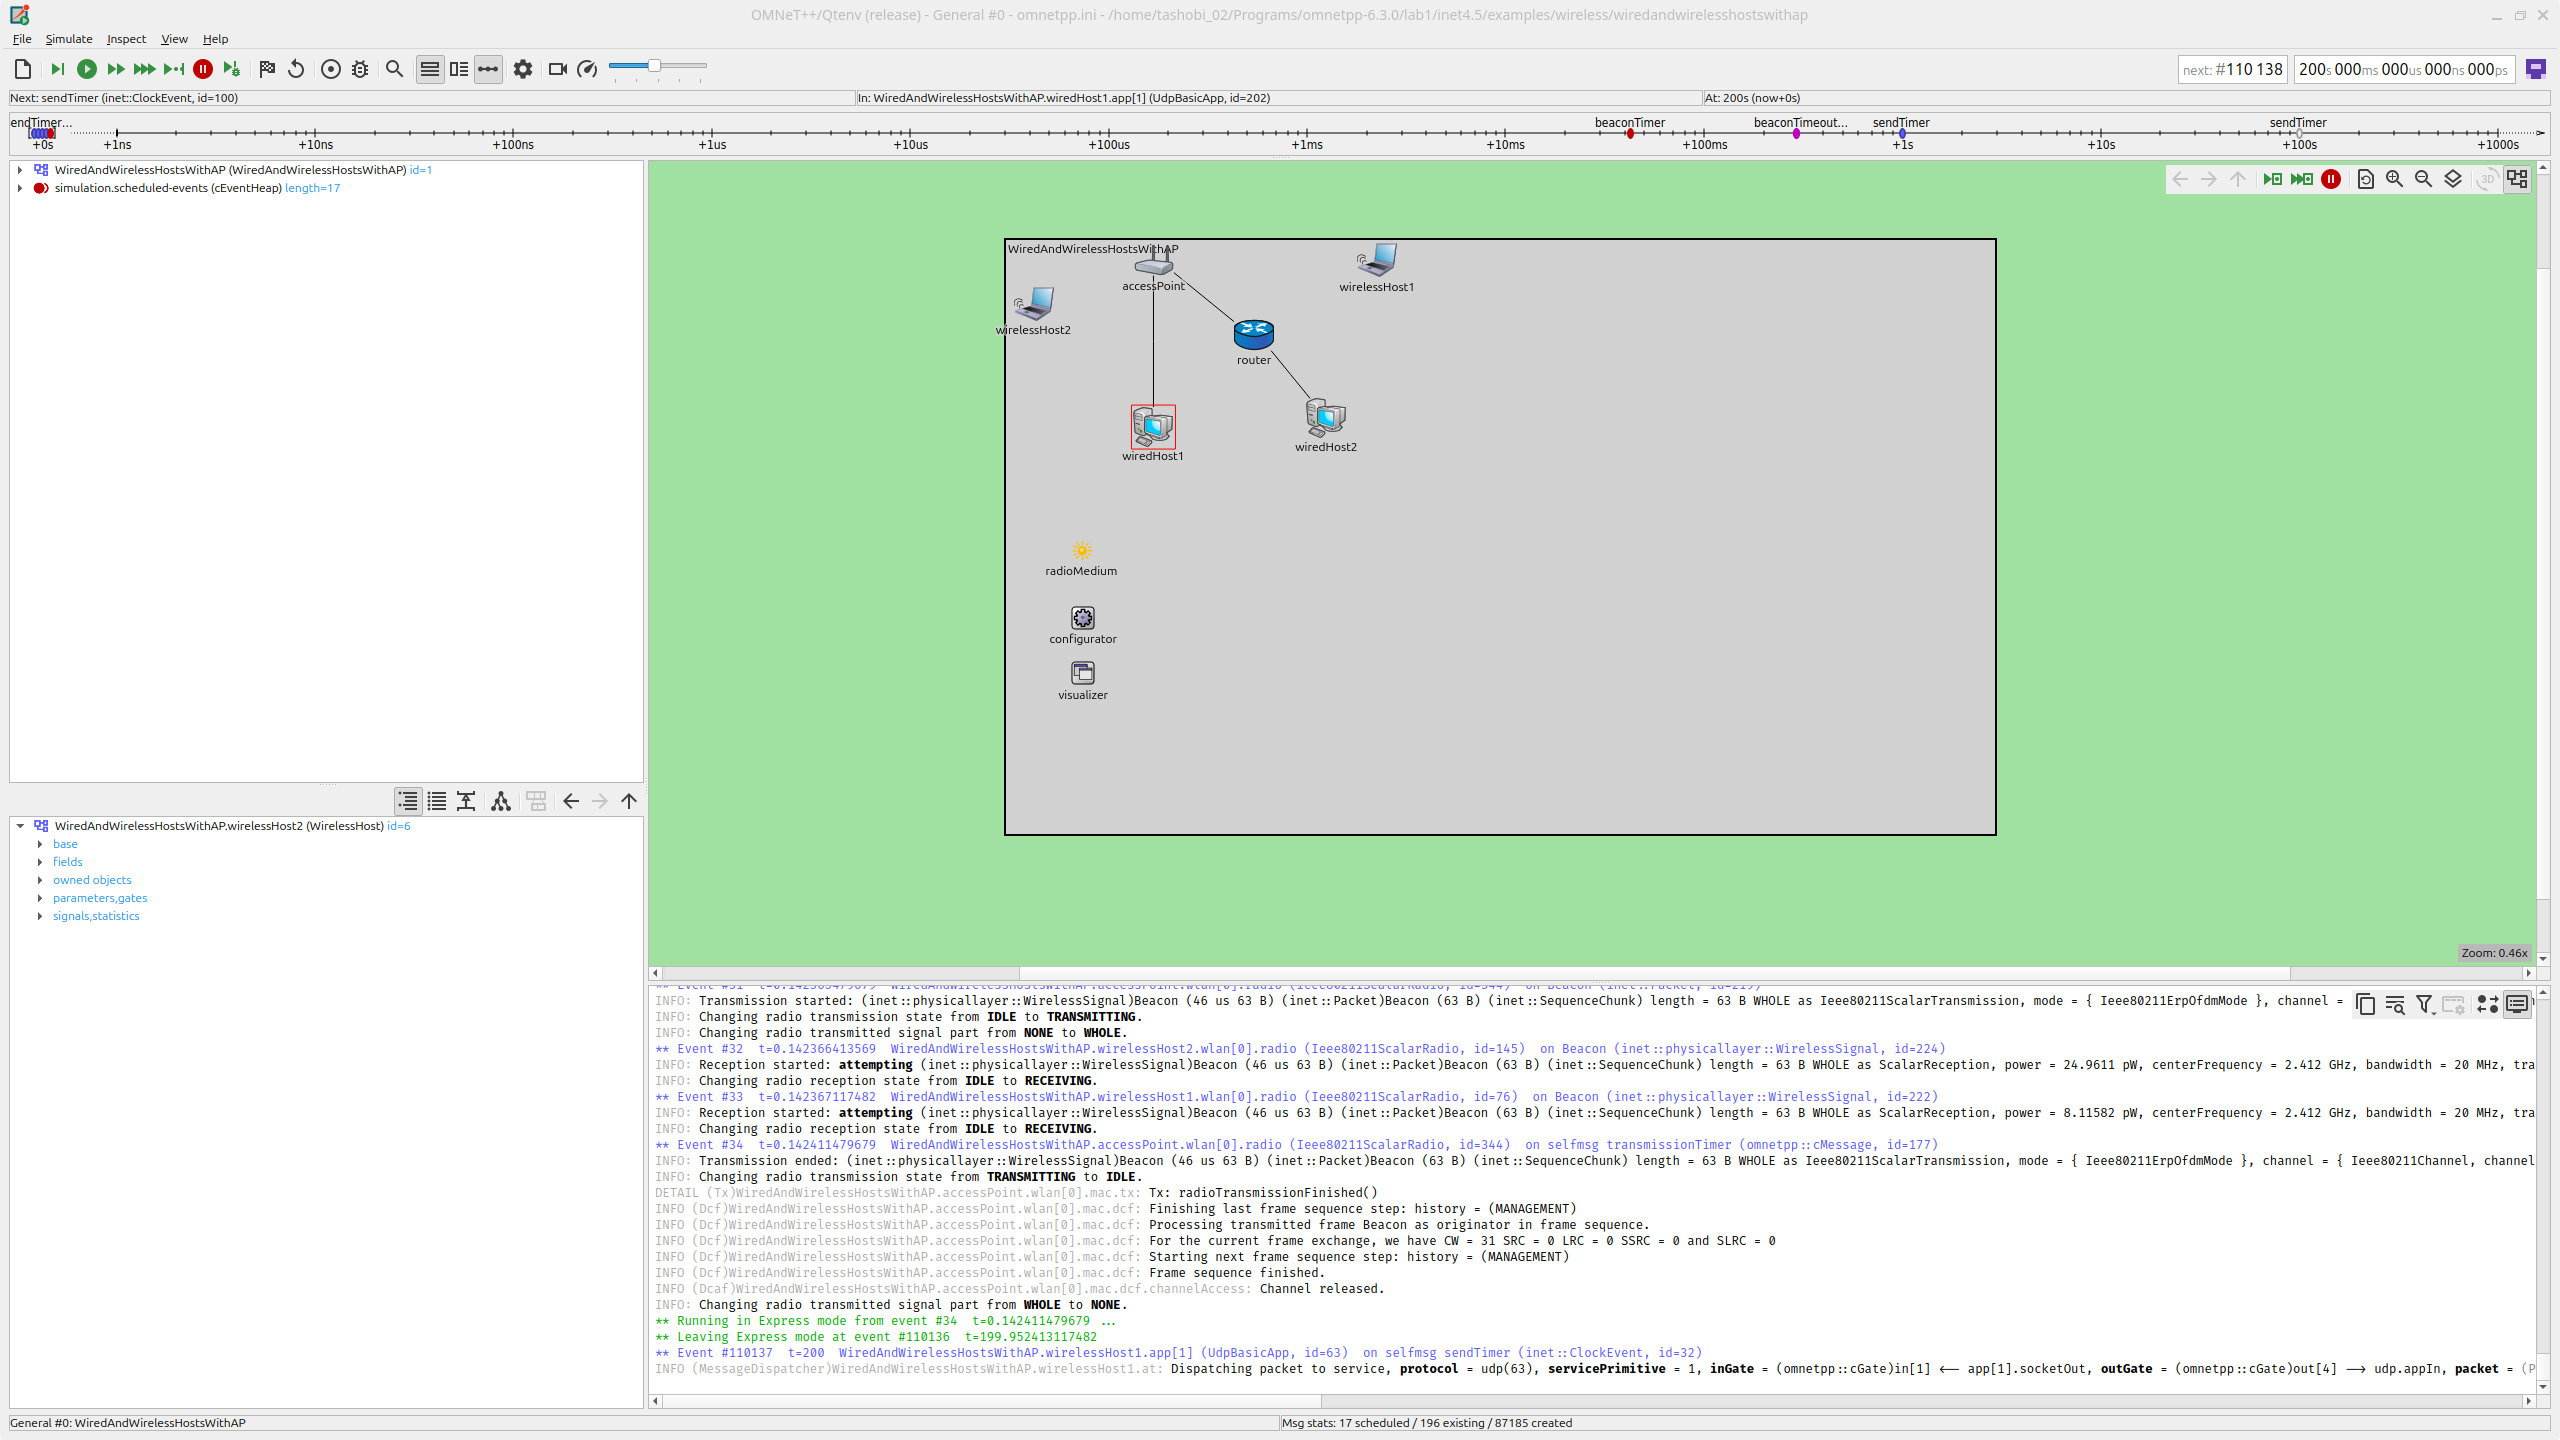
\includegraphics[width=0.9\linewidth]{Figures/fig3.png}
        \caption{Qtenv screenshot showing wirelessHost2 near the access point.}
    \end{figure}
\end{enumerate}

\subsection{Task 03: Add a Third Wired Host and a New Application}
\textbf{Background:} Extend the wired side by adding wiredHost3 and configure app[3] on every host to send traffic to wiredHost3.

\textbf{Required Modifications (NED file):}
\begin{enumerate}
    \item Add a new submodule wiredHost3 of type StandardHost at @display("p=412,140").
    \item Connect wiredHost3 to the router using Eth100M: wiredHost3.ethg++ <--> Eth100M <--> router.ethg++.
\end{enumerate}

\textbf{Required Modifications (INI file):}
\begin{enumerate}
    \item Change numApps from 3 to 4 for all hosts.
    \item app[0] remains UdpEchoApp on port 1000 (explain why in your report).
    \item app[1] and app[2] keep their original destinations.
    \item Configure app[3] on every host to send to wiredHost3 with destPort = 1000, messageLength = 200B, sendInterval = 2s, stopTime = 300s.
    \item Set wiredHost3 app[1] destination to "wiredHost1" and app[2] to "wirelessHost1". Set app[3] to "wiredHost2".
\end{enumerate}

\textbf{Analysis Questions:}
\begin{enumerate}
    \item The line **.*Host*.app[0].typename = "UdpEchoApp" was not changed, yet app[0] on wiredHost3 is automatically set to UdpEchoApp. Why does this happen? Reference the wildcard and specificity rules.\\
    \textbf{Answer:}\\
    Because of the wildcard specificity rule. The line **.*Host*.app[0].typename = "UdpEchoApp" targets every host's app[0] by exact index. Since wiredHost3's name contains "Host", this rule applies to it automatically -- no extra line needed. The wildcard app[*].typename = "UdpBasicApp" is lower priority, so app[0] keeps UdpEchoApp.
    \item What is the total number of packets per second generated across the entire network? Show your working.\\
    \textbf{Answer:}\\
    4 hosts $\times$ 3 sending apps each (app[1], app[2], app[3]) -- but app[3] sends every 2s (0.5 pkt/s), while app[1] and app[2] send every 1s (1 pkt/s each).\\
    Per host: 1 + 1 + 0.5 = 2.5 packets/second.\\
    Total network: 4 $\times$ 2.5 = 10 packets/second.
    \item In Qtenv, describe the path a packet takes from wiredHost3 to wirelessHost1. Name every intermediate device it passes through.\\
    \textbf{Answer:}\\
    wiredHost3 $\rightarrow$ (Eth100M cable) $\rightarrow$ router $\rightarrow$ (Eth100M cable) $\rightarrow$ accessPoint $\rightarrow$ (Wi-Fi via radioMedium) $\rightarrow$ wirelessHost1.\\
    Intermediate devices: router, accessPoint. The router routes the IP packet, and the accessPoint bridges from wired Ethernet to the wireless radio.
    \begin{figure}[H]
        \centering
        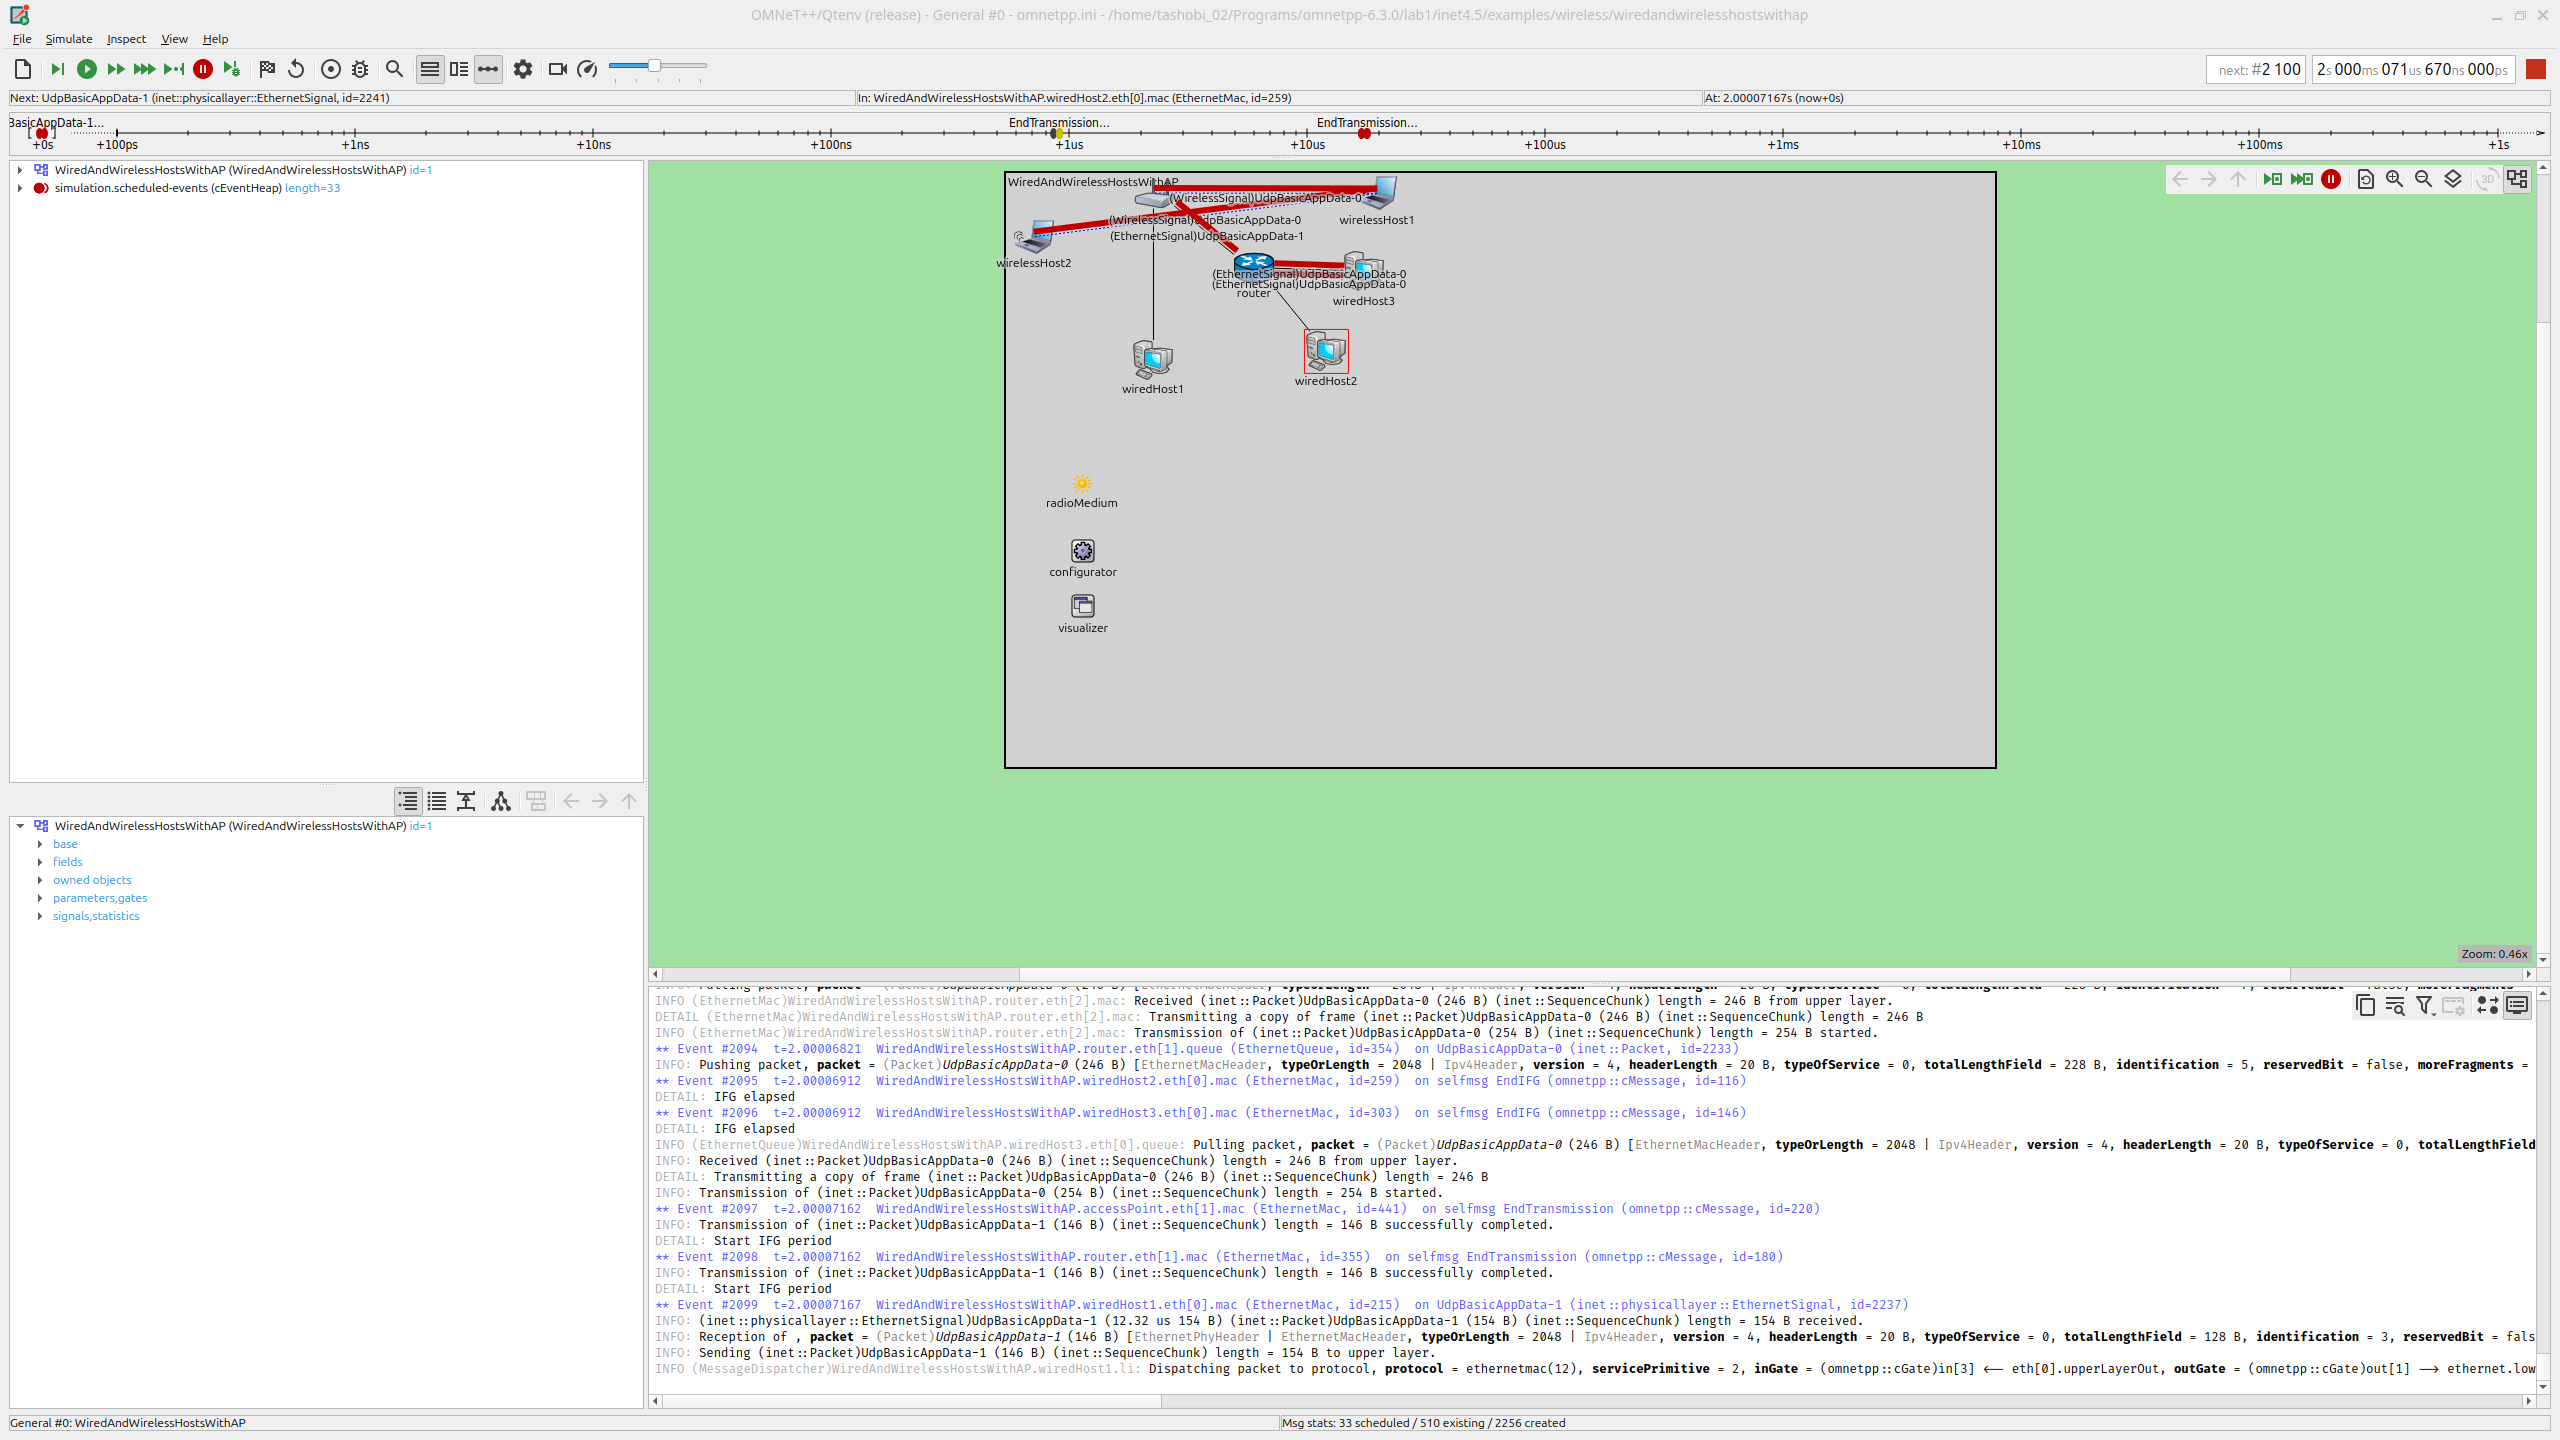
\includegraphics[width=0.9\linewidth]{Figures/fig4.png}
        \caption{Qtenv screenshot showing wiredHost3 connected to the router.}
    \end{figure}
\end{enumerate}

\subsection{Task 04: Staggered Traffic and Selective Recording}
\textbf{Background:} Introduce staggered start times, randomize send intervals, and selectively enable vector recording.

\textbf{Required Modifications (INI file only):}
\begin{enumerate}
    \item Disable global vector recording and enable it only for wiredHost1 and the router.
    \item Stagger the start times of the sending apps so that hosts begin transmitting at different simulated times.
    \item Change the send interval of all sending apps from fixed 1s to exponential(1s).
    \item Keep all other parameters (packet size, stop time, simulation limit) at their original values.
\end{enumerate}

\textbf{Analysis Questions:}
\begin{enumerate}
    \item At simulated time t = 12 s, which hosts are actively sending packets and which are not? Justify your answer using the start times.\\
    \textbf{Answer:}\\
    Apps started by t = 12 s:\\
    wiredHost1.app[1] (0s) -- active\\
    wiredHost1.app[2] (5s) -- active\\
    wiredHost2.app[1] (10s) -- active\\
    wiredHost2.app[2] (15s) -- not yet\\
    wirelessHost1.app[1] (20s) -- not yet\\
    wirelessHost1.app[2] (25s) -- not yet\\
    Active senders at t = 12 s: wiredHost1 (both apps) and wiredHost2 (app[1]). wirelessHost1 has not started yet.
    \item Why is exponential(1s) a more realistic model for network traffic than a fixed 1s interval? What real-world phenomenon does this distribution model?\\
    \textbf{Answer:}\\
    Fixed 1s intervals produce perfectly regular, deterministic traffic -- real networks do not behave this way. The exponential distribution models a memoryless Poisson arrival process, meaning each new packet is equally likely to arrive at any moment regardless of when the last one did. This matches bursty user traffic (e.g., multiple requests followed by a quiet period) and also models TCP's bursty retransmission behavior. The exponential distribution with mean 1s is the inter-arrival time distribution of a Poisson process, which is the standard model for network traffic in queueing theory.
    \item Why is it useful to disable vector recording globally and enable it only for selected modules? What problem does this solve in large simulations?\\
    \textbf{Answer:}\\
    Vector recording writes time-series data (every packet sent, every queue length sample) to disk for every module. In large simulations, this creates enormous result files and slows the simulation down significantly. Disabling it globally and enabling it only for wiredHost1 and the router captures the data you care about while keeping file size manageable and simulation performance reasonable.
    \item In Qtenv, take a screenshot at t = 22 s. Which hosts should be visible as active senders at that moment? Does your screenshot confirm this?\\
    \textbf{Answer:}\\
    At t = 22 s, all apps with startTime $\le$ 22 s are active: wiredHost1.app[1] (0s), wiredHost1.app[2] (5s), wiredHost2.app[1] (10s), wiredHost2.app[2] (15s), and wirelessHost1.app[1] (20s). wirelessHost1.app[2] (25s) has not started yet. All three hosts are sending at least one packet stream, and the screenshot confirms this.
    \begin{figure}[H]
        \centering
        \begin{subfigure}{0.9\linewidth}
            \centering
            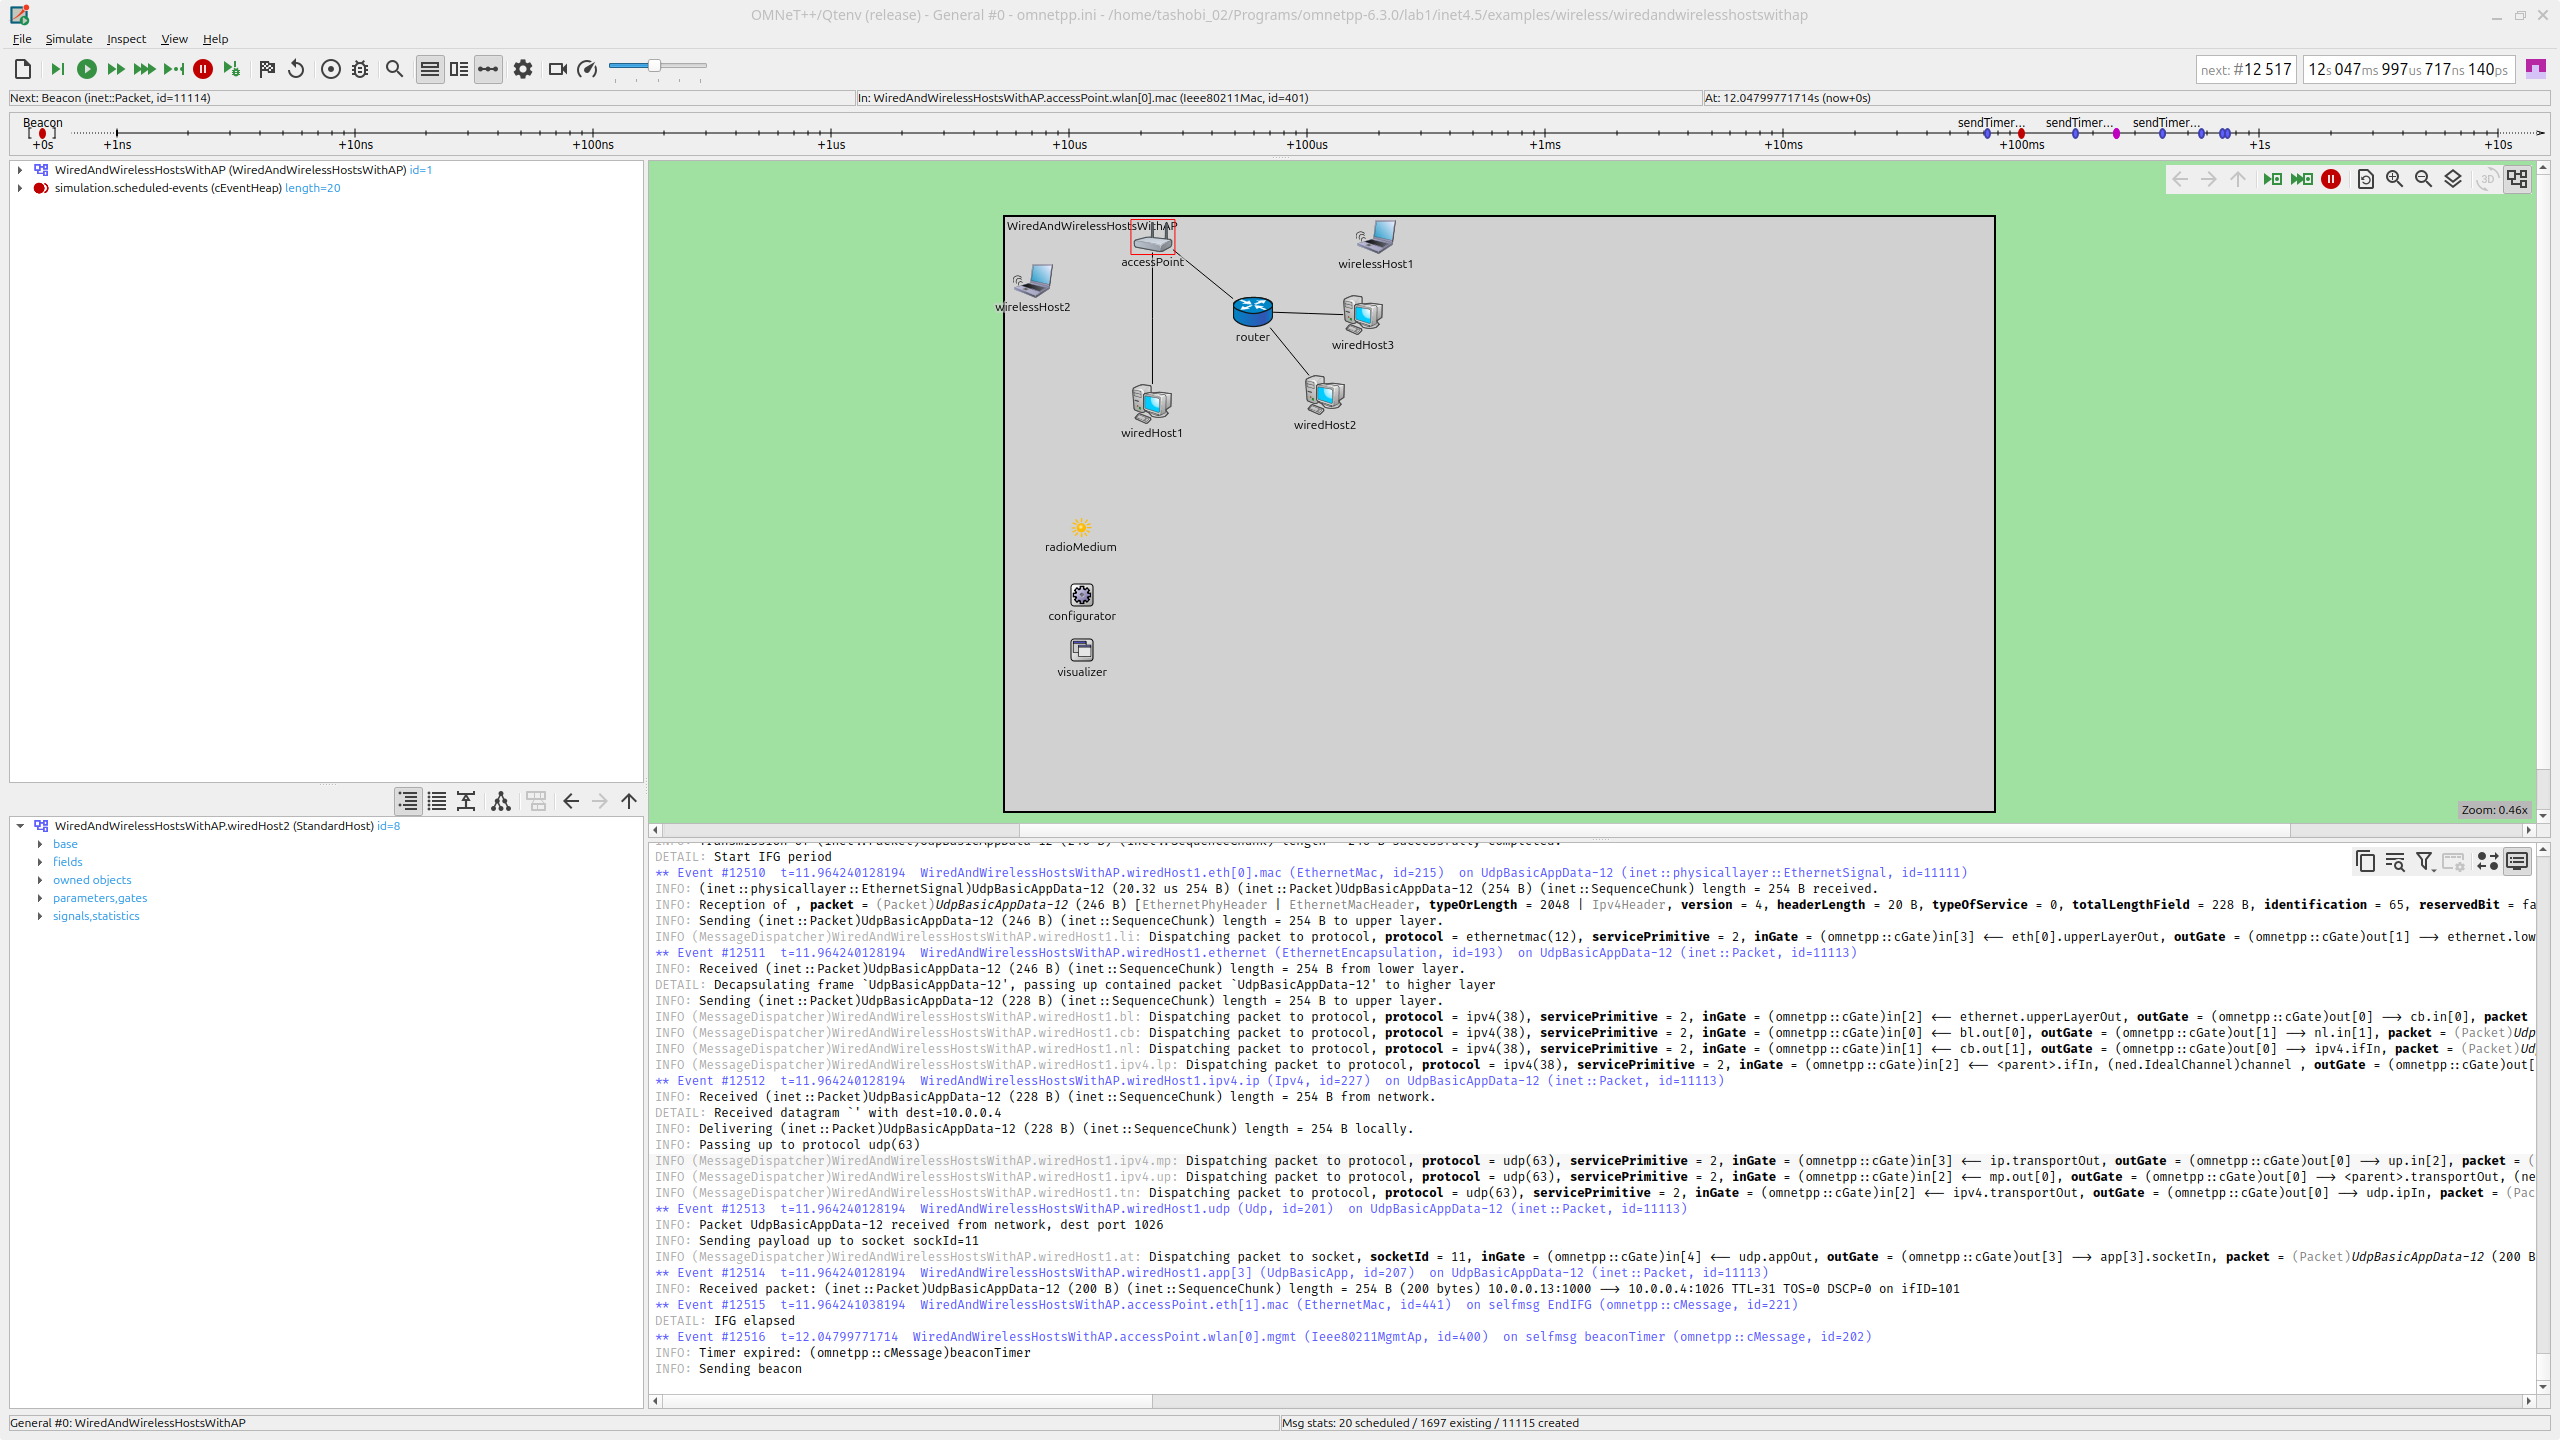
\includegraphics[width=\linewidth]{Figures/fig5.png}
            \caption{t = 12 s}
        \end{subfigure}
        \vspace{6pt}
        \begin{subfigure}{0.9\linewidth}
            \centering
            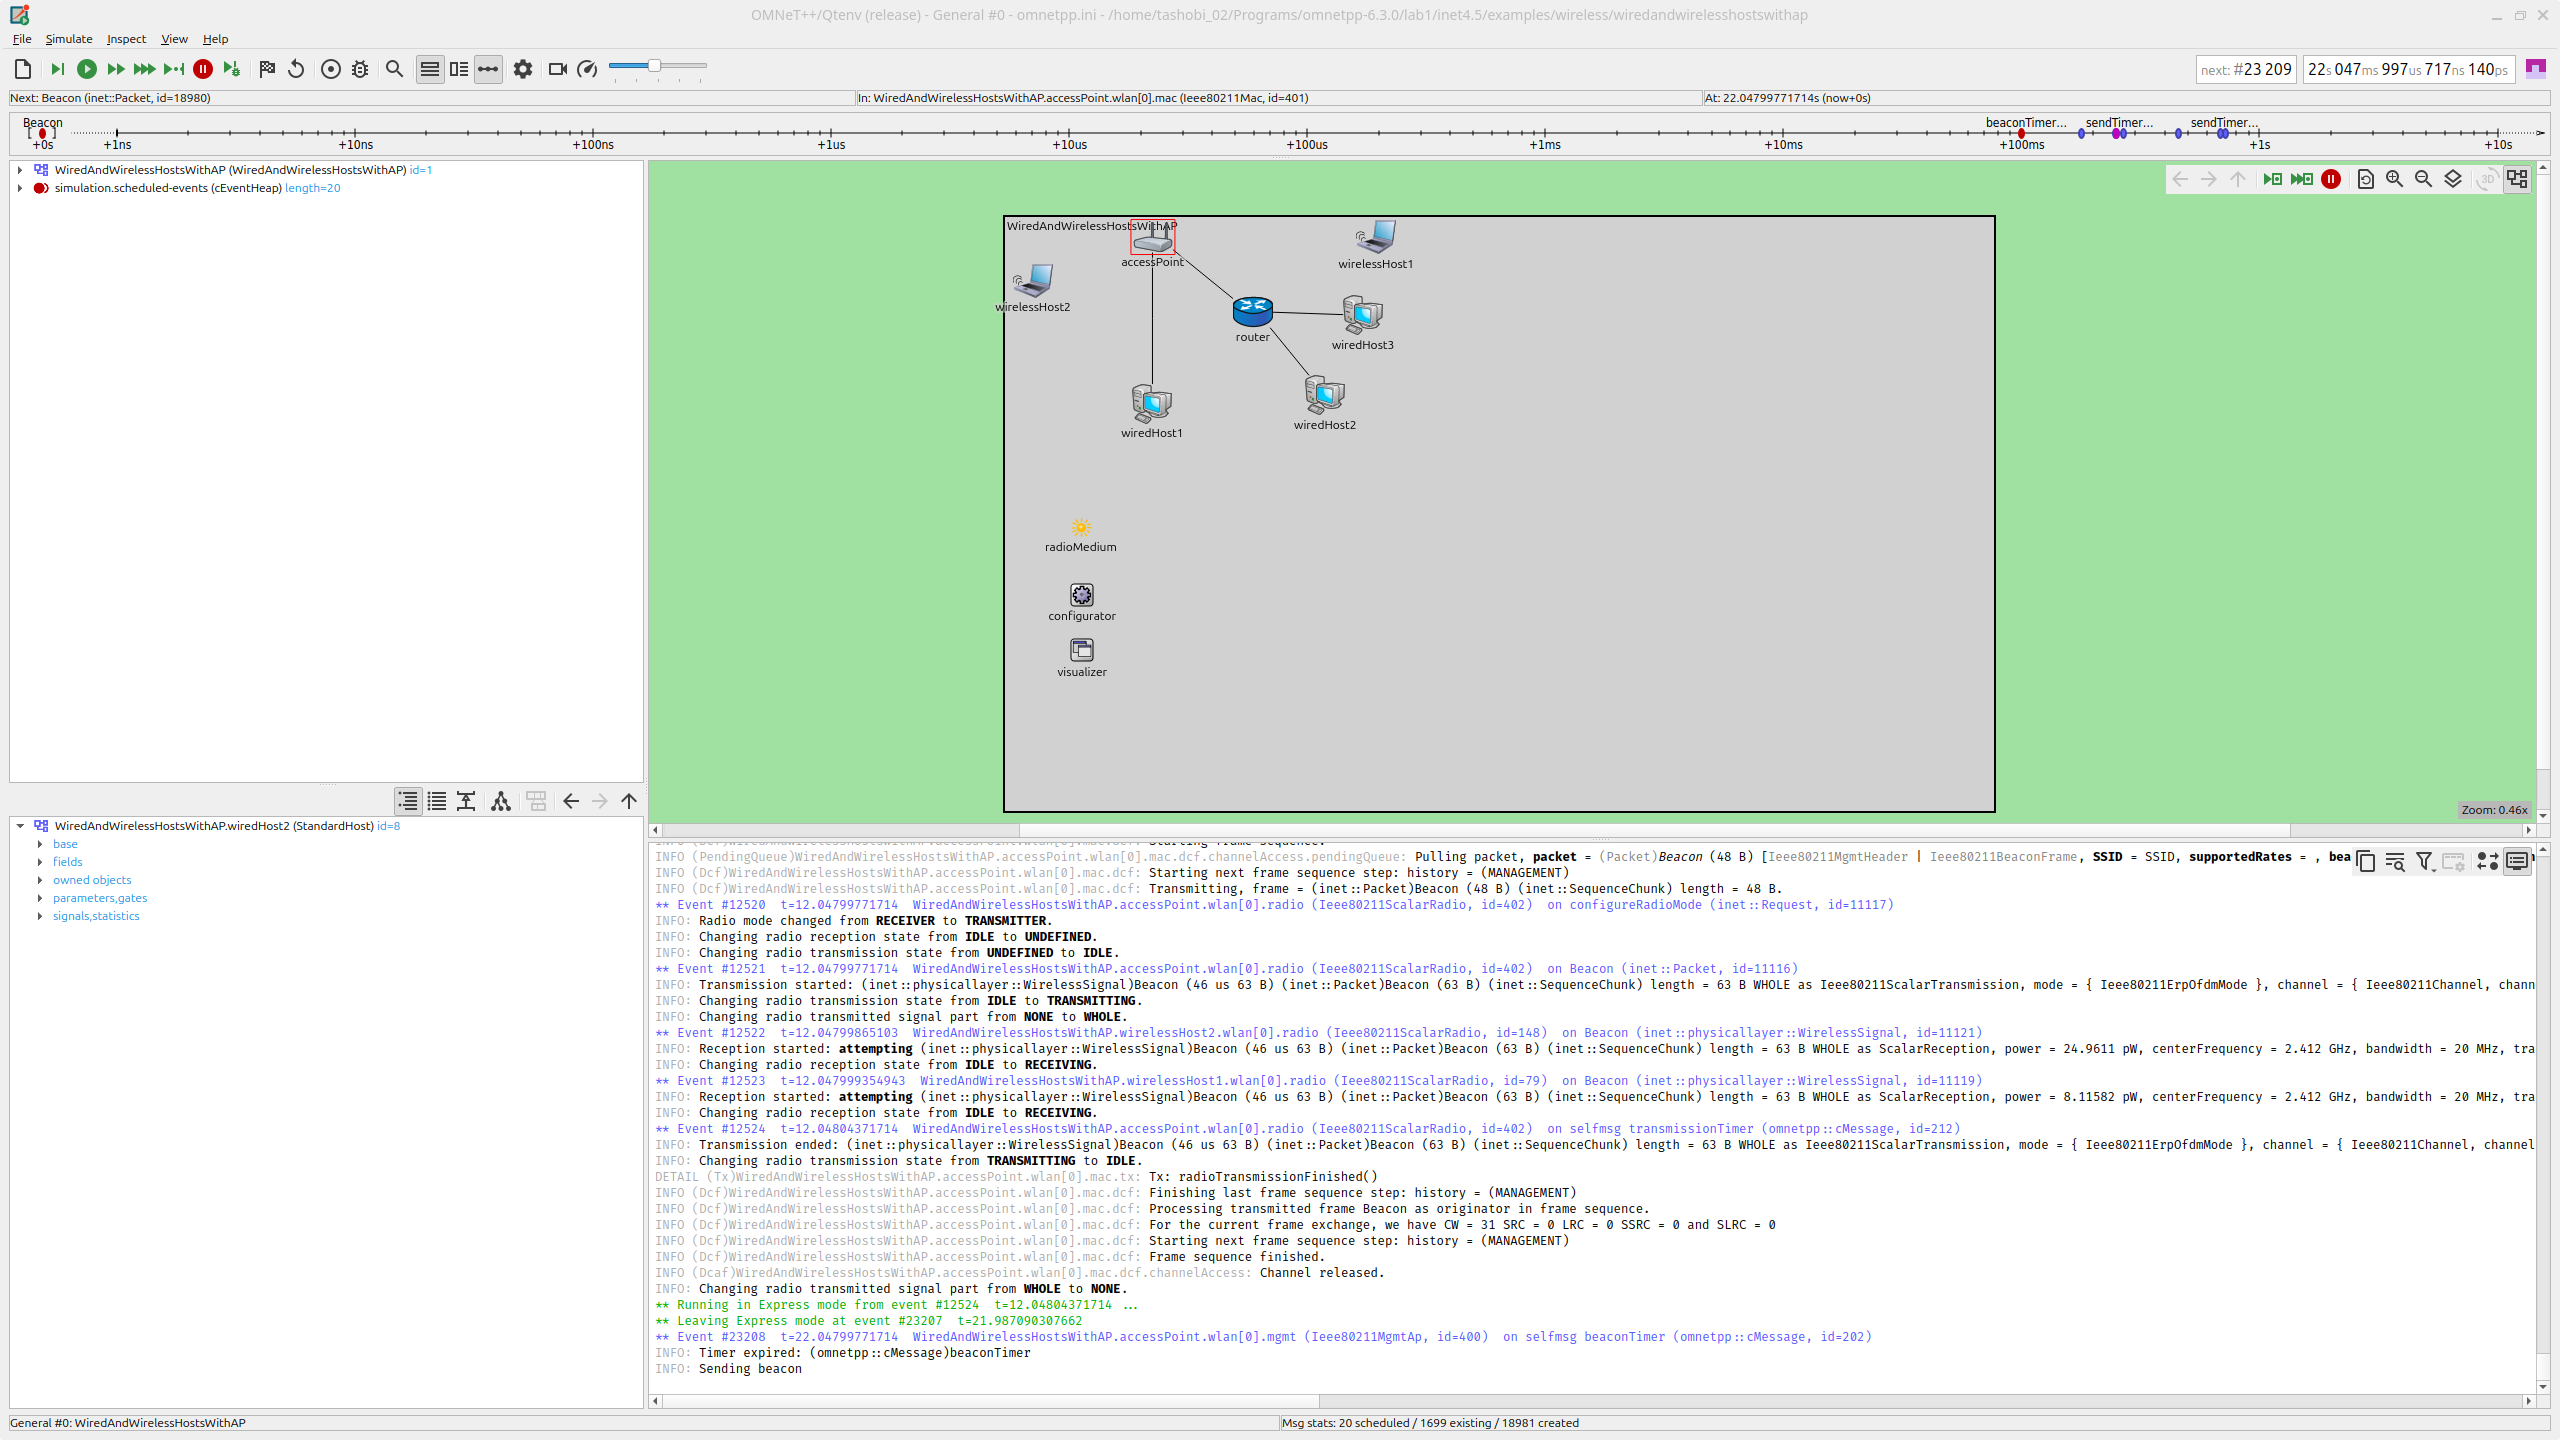
\includegraphics[width=\linewidth]{Figures/fig6.png}
            \caption{t = 22 s}
        \end{subfigure}
        \caption{Qtenv screenshots for Task 04.}
    \end{figure}
\end{enumerate}

\end{document}
